\documentclass[10pt, a4paper]{article}
\usepackage[utf8]{inputenc}
\usepackage{listings}
\usepackage{pgfplotstable}
\pgfplotsset{compat=1.13}

\title{Heuristic Analysis}
\author{Nathan Findley}
\date{March 2017}

\begin{document}

\maketitle
\tableofcontents

\begin{abstract}
	Abstract
\end{abstract}

\section{Non-Heuristic Solutions}

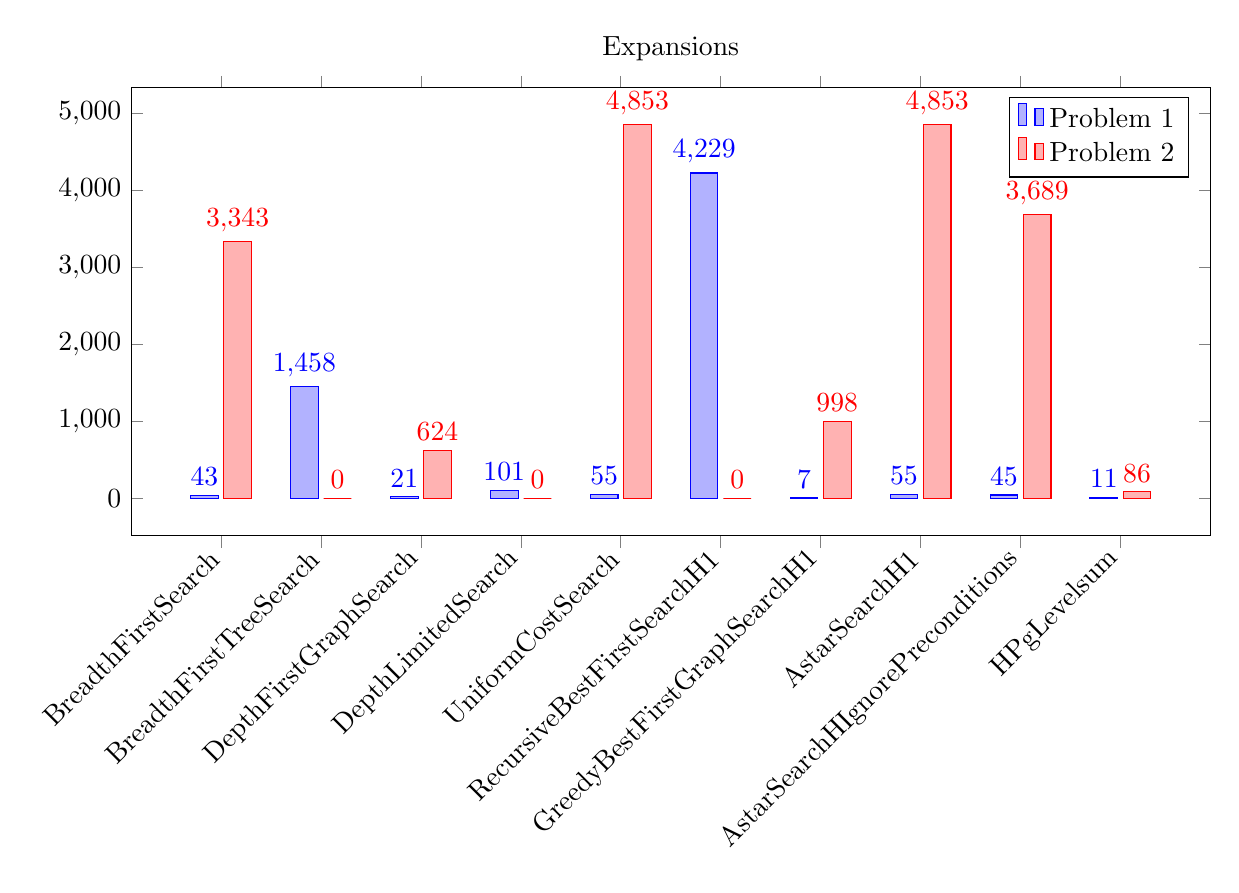
\begin{tikzpicture}
	\begin{axis}[
			title={Expansions},
			ybar,
			symbolic x coords={BreadthFirstSearch,BreadthFirstTreeSearch,DepthFirstGraphSearch,DepthLimitedSearch,UniformCostSearch,RecursiveBestFirstSearchH1,GreedyBestFirstGraphSearchH1,AstarSearchH1,AstarSearchHIgnorePreconditions,HPgLevelsum},
			x post scale=2,
			x tick label style={rotate=45,anchor=east},
			nodes near coords
			]

		\addplot table {
			X Y
		BreadthFirstSearch 43
		BreadthFirstTreeSearch 1458
		DepthFirstGraphSearch 21
		DepthLimitedSearch 101
		UniformCostSearch 55
		RecursiveBestFirstSearchH1 4229
		GreedyBestFirstGraphSearchH1 7
		AstarSearchH1 55
		AstarSearchHIgnorePreconditions 45
		HPgLevelsum 11
		};

		\addplot table {
			X Y
			BreadthFirstSearch 3343
			BreadthFirstTreeSearch 0
			DepthFirstGraphSearch 624
			DepthLimitedSearch 0
			UniformCostSearch 4853
			RecursiveBestFirstSearchH1 0
			GreedyBestFirstGraphSearchH1 998
			AstarSearchH1 4853
			AstarSearchHIgnorePreconditions 3689
			HPgLevelsum 86
			};

		\addlegendentry{Problem 1}
		\addlegendentry{Problem 2}
		\addlegendentry{Problem 3}
	\end{axis}
\end{tikzpicture}

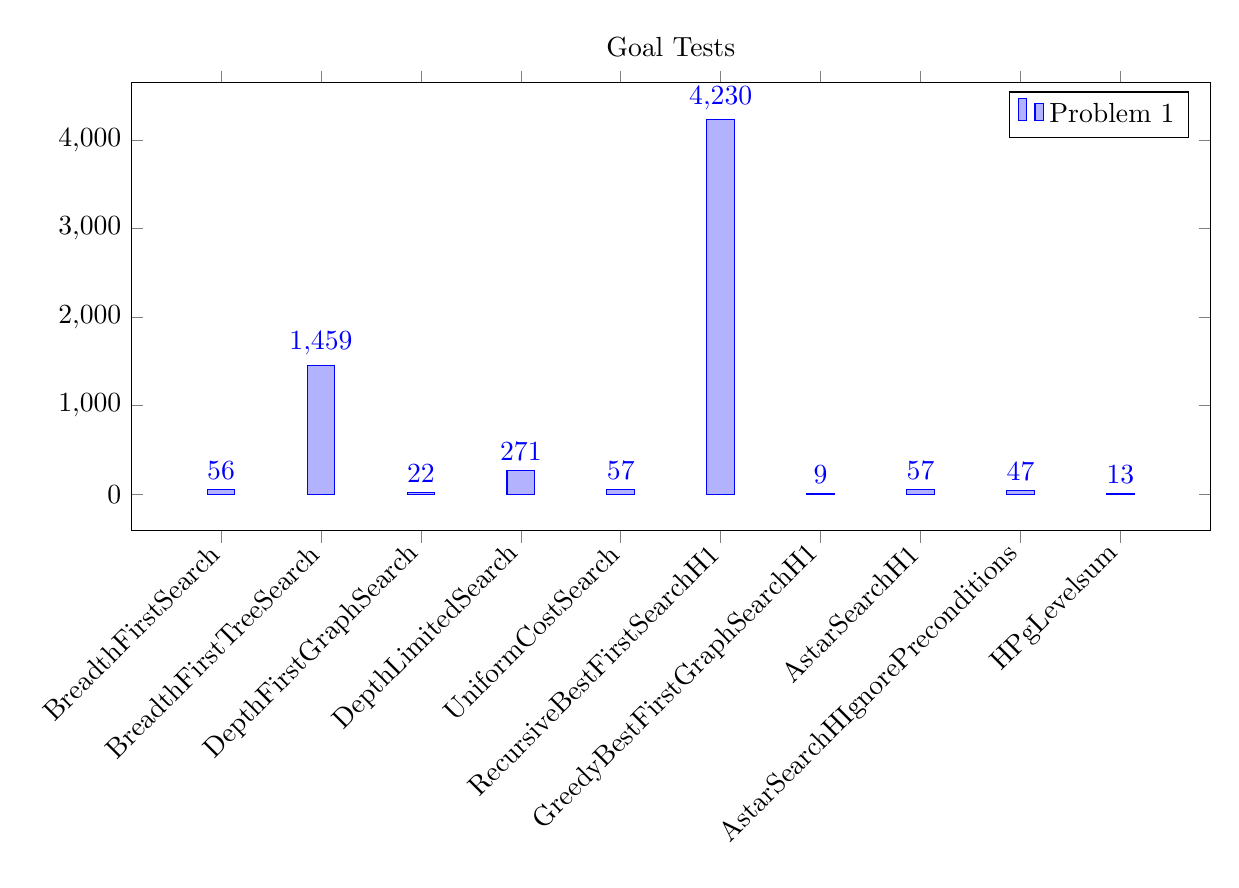
\begin{tikzpicture}
	\begin{axis}[
			title={Goal Tests},
			ybar,
			symbolic x coords={BreadthFirstSearch,BreadthFirstTreeSearch,DepthFirstGraphSearch,DepthLimitedSearch,UniformCostSearch,RecursiveBestFirstSearchH1,GreedyBestFirstGraphSearchH1,AstarSearchH1,AstarSearchHIgnorePreconditions,HPgLevelsum},
			x post scale=2,
			x tick label style={rotate=45,anchor=east},
			nodes near coords
			]

		\addplot table {
			X Y
		BreadthFirstSearch 56
		BreadthFirstTreeSearch 1459
		DepthFirstGraphSearch 22
		DepthLimitedSearch 271
		UniformCostSearch 57
		RecursiveBestFirstSearchH1 4230
		GreedyBestFirstGraphSearchH1 9
		AstarSearchH1 57
		AstarSearchHIgnorePreconditions 47
		HPgLevelsum 13
		};
		\addlegendentry{Problem 1}
		\addlegendentry{Problem 2}
		\addlegendentry{Problem 3}
	\end{axis}
\end{tikzpicture}

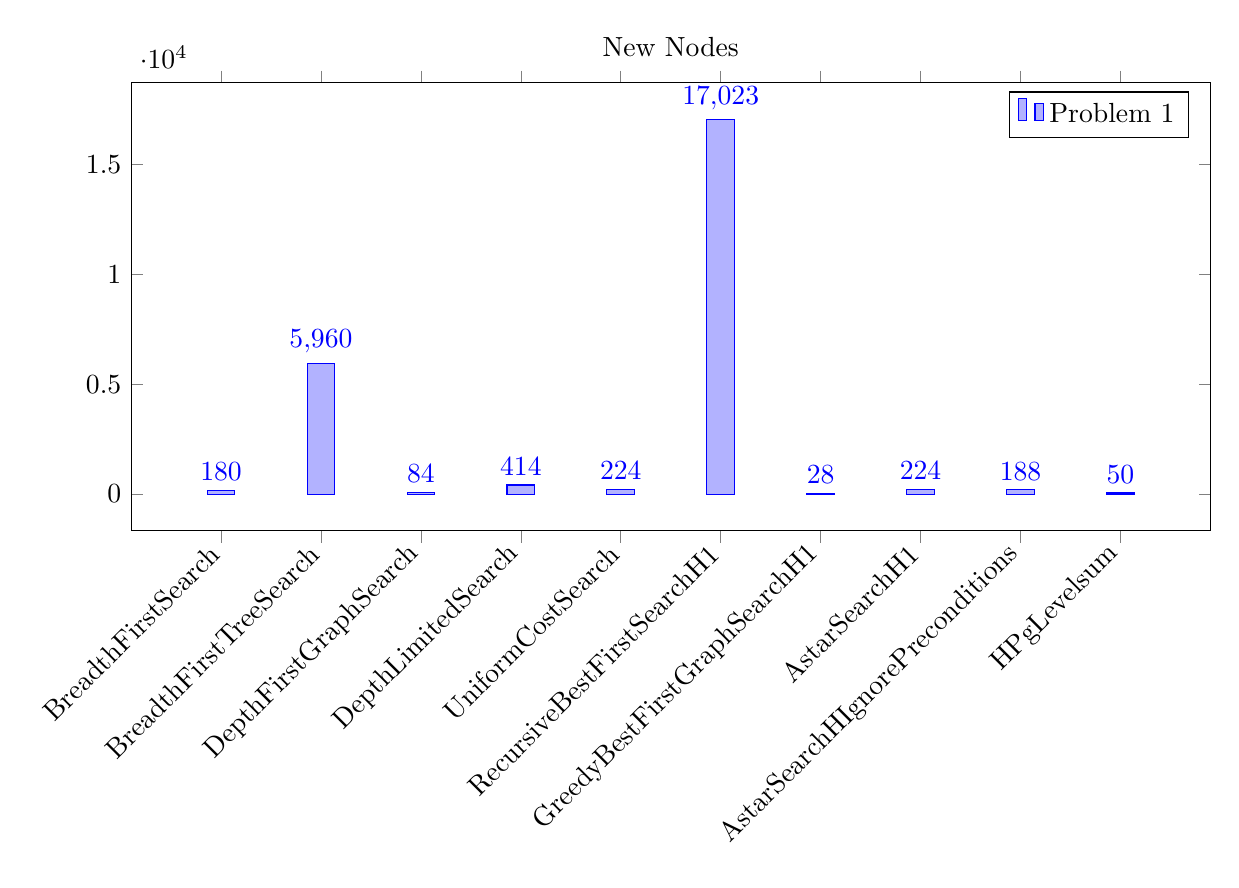
\begin{tikzpicture}
	\begin{axis}[
			title={New Nodes},
			ybar,
			symbolic x coords={BreadthFirstSearch,BreadthFirstTreeSearch,DepthFirstGraphSearch,DepthLimitedSearch,UniformCostSearch,RecursiveBestFirstSearchH1,GreedyBestFirstGraphSearchH1,AstarSearchH1,AstarSearchHIgnorePreconditions,HPgLevelsum},
			x post scale=2,
			x tick label style={rotate=45,anchor=east},
			nodes near coords
			]

		\addplot table {
			X Y
		BreadthFirstSearch 180
		BreadthFirstTreeSearch 5960
		DepthFirstGraphSearch 84
		DepthLimitedSearch 414
		UniformCostSearch 224
		RecursiveBestFirstSearchH1 17023
		GreedyBestFirstGraphSearchH1 28
		AstarSearchH1 224
		AstarSearchHIgnorePreconditions 188
		HPgLevelsum 50
		};
		\addlegendentry{Problem 1}
		\addlegendentry{Problem 2}
		\addlegendentry{Problem 3}
	\end{axis}
\end{tikzpicture}

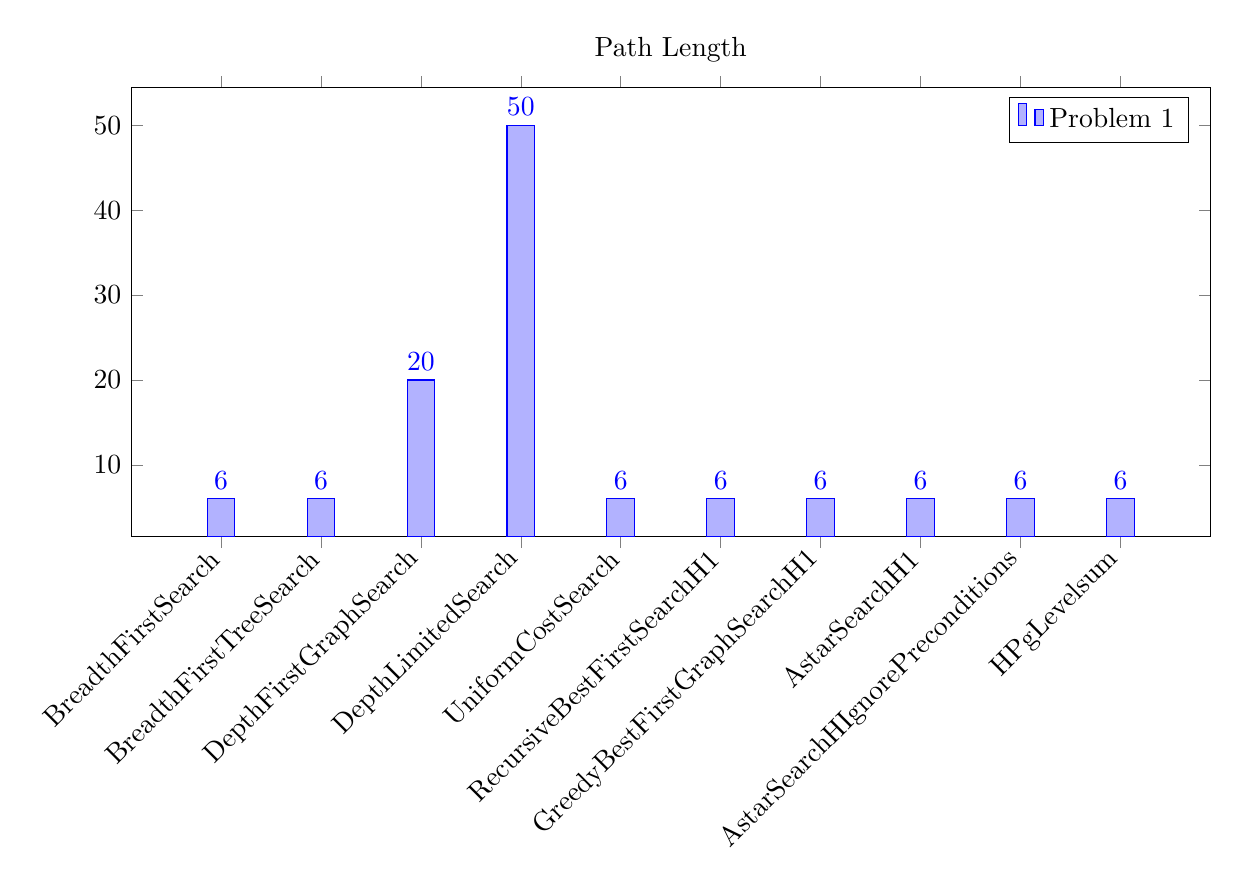
\begin{tikzpicture}
	\begin{axis}[
			title={Path Length},
			ybar,
			symbolic x coords={BreadthFirstSearch,BreadthFirstTreeSearch,DepthFirstGraphSearch,DepthLimitedSearch,UniformCostSearch,RecursiveBestFirstSearchH1,GreedyBestFirstGraphSearchH1,AstarSearchH1,AstarSearchHIgnorePreconditions,HPgLevelsum},
			x post scale=2,
			x tick label style={rotate=45,anchor=east},
			nodes near coords
			]

		\addplot table {
			X Y
		BreadthFirstSearch 6
		BreadthFirstTreeSearch 6
		DepthFirstGraphSearch 20
		DepthLimitedSearch 50
		UniformCostSearch 6
		RecursiveBestFirstSearchH1 6
		GreedyBestFirstGraphSearchH1 6
		AstarSearchH1 6
		AstarSearchHIgnorePreconditions 6
		HPgLevelsum 6
		};
		\addlegendentry{Problem 1}
		\addlegendentry{Problem 2}
		\addlegendentry{Problem 3}
	\end{axis}
\end{tikzpicture}


\section{Consume The Opponent's Movement Space}

Favor moves where the player encroaches on the opponent's moves or follow them around
the board. Also uses the idea of trying to stop an opponent that suddenly has limited movement.

\begin{lstlisting}[language=Python]
		playerMoves = game.get_legal_moves(player)
		opponentMoves = game.get_legal_moves(game.get_opponent(player))
		if len(opponentMoves) == 1:
				for o in opponentMoves:
						for p in playerMoves:
								if o == p:
										return float("+inf")

		matchedMoves = 0
		centerAt = board_center(game)
		for o in opponentMoves:
				for p in playerMoves:
						if o == p:
								matchedMoves += 10
		if matchedMoves > 0:
				return float(matchedMoves)

		playerAt = game.get_player_location(player)
		opponentAt = game.get_player_location(game.get_opponent(player))

		xDiff = playerAt[0] - opponentAt[0]
		yDiff = playerAt[1] - opponentAt[1]
		denom = float(xDiff*xDiff + yDiff*yDiff)
		if denom == 0:
				return float("+inf")
		return float(1.0/denom)
\end{lstlisting}

\begin{verbatim}
*************************
 Evaluating: ID_Improved 
*************************

Playing Matches:
----------
	Match 1: ID_Improved vs   Random    	Result: 184 to 16
	Match 2: ID_Improved vs   MM_Null   	Result: 174 to 26
	Match 3: ID_Improved vs   MM_Open   	Result: 157 to 43
	Match 4: ID_Improved vs MM_Improved 	Result: 141 to 59
	Match 5: ID_Improved vs   AB_Null   	Result: 161 to 39
	Match 6: ID_Improved vs   AB_Open   	Result: 136 to 64
	Match 7: ID_Improved vs AB_Improved 	Result: 123 to 77


Results:
----------
ID_Improved         76.86%

*************************
	 Evaluating: Student   
*************************

Playing Matches:
----------
	Match 1:   Student   vs   Random    	Result: 181 to 19
	Match 2:   Student   vs   MM_Null   	Result: 168 to 32
	Match 3:   Student   vs   MM_Open   	Result: 146 to 54
	Match 4:   Student   vs MM_Improved 	Result: 138 to 62
	Match 5:   Student   vs   AB_Null   	Result: 156 to 44
	Match 6:   Student   vs   AB_Open   	Result: 127 to 73
	Match 7:   Student   vs AB_Improved 	Result: 121 to 79


Results:
----------
Student             74.07%
\end{verbatim}

Seeing that the value drops below 75\% is not encouraging.

\section{Remain Near The Center}

Favor moves that position the player closer to the center of the board.

\begin{lstlisting}[language=Python]
		centerAt = board_center(game)
		playerAt = game.get_player_location(player)

		xDiff = playerAt[0] - centerAt[0]
		yDiff = playerAt[1] - centerAt[1]
		denom = float(xDiff*xDiff + yDiff*yDiff)
		if denom == 0:
				return float("+inf")
		return float(1.0/denom)
\end{lstlisting}

\begin{verbatim}
*************************
 Evaluating: ID_Improved 
*************************

Playing Matches:
----------
	Match 1: ID_Improved vs   Random    	Result: 179 to 21
	Match 2: ID_Improved vs   MM_Null   	Result: 176 to 24
	Match 3: ID_Improved vs   MM_Open   	Result: 148 to 52
	Match 4: ID_Improved vs MM_Improved 	Result: 146 to 54
	Match 5: ID_Improved vs   AB_Null   	Result: 154 to 46
	Match 6: ID_Improved vs   AB_Open   	Result: 127 to 73
	Match 7: ID_Improved vs AB_Improved 	Result: 126 to 74


Results:
----------
ID_Improved         75.43%

*************************
	 Evaluating: Student   
*************************

Playing Matches:
----------
	Match 1:   Student   vs   Random    	Result: 180 to 20
	Match 2:   Student   vs   MM_Null   	Result: 162 to 38
	Match 3:   Student   vs   MM_Open   	Result: 138 to 62
	Match 4:   Student   vs MM_Improved 	Result: 131 to 69
	Match 5:   Student   vs   AB_Null   	Result: 142 to 58
	Match 6:   Student   vs   AB_Open   	Result: 138 to 62
	Match 7:   Student   vs AB_Improved 	Result: 127 to 73


Results:
----------
Student             72.71%
\end{verbatim}

This ends up being the most disappointing set of results.  This is clearly not
a winning strategy.

\section{Central Hover Followed By Most Moves}

Favor moves that position the player closer to the center of the board until the game board is 40\% full.
Otherwise, simply move as ID Improved would giving heavy weight on a set of moves that can pinch an opponent.

\begin{lstlisting}[language=Python]
		blanks = game.get_blank_spaces()
		if len(blanks) > (3*game.width*game.height/5):
				centerAt = board_center(game)
				playerAt = game.get_player_location(player)
				xDiff = playerAt[0] - centerAt[0]
				yDiff = playerAt[1] - centerAt[1]
				denom = float(xDiff*xDiff + yDiff*yDiff)
				if denom == 0:
						return float("+inf")
				return float(1.0/denom)

		playerMoves = game.get_legal_moves(player)
		opponentMoves = game.get_legal_moves(game.get_opponent(player))
		if len(opponentMoves) == 1:
				for o in opponentMoves:
						for p in playerMoves:
								if o == p:
										return float("+inf")

		return float(len(game.get_legal_moves(player))-
			len(game.get_legal_moves(game.get_opponent(player))))
\end{lstlisting}

\begin{verbatim}
*************************
 Evaluating: ID_Improved 
*************************

Playing Matches:
----------
	Match 1: ID_Improved vs   Random    	Result: 180 to 20
	Match 2: ID_Improved vs   MM_Null   	Result: 175 to 25
	Match 3: ID_Improved vs   MM_Open   	Result: 155 to 45
	Match 4: ID_Improved vs MM_Improved 	Result: 148 to 52
	Match 5: ID_Improved vs   AB_Null   	Result: 164 to 36
	Match 6: ID_Improved vs   AB_Open   	Result: 134 to 66
	Match 7: ID_Improved vs AB_Improved 	Result: 126 to 74


Results:
----------
ID_Improved         77.29%

*************************
	 Evaluating: Student   
*************************

Playing Matches:
----------
	Match 1:   Student   vs   Random    	Result: 189 to 11
	Match 2:   Student   vs   MM_Null   	Result: 177 to 23
	Match 3:   Student   vs   MM_Open   	Result: 159 to 41
	Match 4:   Student   vs MM_Improved 	Result: 149 to 51
	Match 5:   Student   vs   AB_Null   	Result: 162 to 38
	Match 6:   Student   vs   AB_Open   	Result: 136 to 64
	Match 7:   Student   vs AB_Improved 	Result: 133 to 67


Results:
----------
Student             78.93%
\end{verbatim}

This is the first time one of my heuristics has outperformed ID Improved.  Considering that this
is a variation of ID Improved's heuristic, perhaps I shouldn't be surprised that it is highly competitive.

\section{Results}

The ID Improved heuristic consistently achieves scores from 75-78\% based on testing.

Among all four contenders, "Central Hover Followed by Most Moves" appears to be the best option.
By initially remaining near the center of the board, it seems
that this should allow for more available moves, permitting more possibility for finding a winning branch.
I like the idea of coming up with strategies that highly favor being able to see "horizon" results 
before they happen, unfortunately I am not sure how to do that in an isolation scenario with chess-like knight movement.
As such, highly favoring a single move that includes the possibility of taking the opponent's final move
is where my strategy stopped in that regard.  Naturally, given that the original ID Improved heuristic
was difficult for me to overcome, incorporating it into a more detailed strategy felt like a good approach.

\section{Beyond Project Scope - Breaking Changes}

The following results were obtained by changing the way that the iterative deepening
evaluates layers above depth == 1.  If one makes the changes below so that greater than and
less than comparisons become strictly greater or strictly less than, the search space is
expanded but the win percentages increase.  Doing this will result in the agent\_test.py
failing so I have not included it in my final result, but this was an interesting accidental
discovery.  This version seems superior particularly since it gives one of the highest win percentages
that any of my testing has yet seen.  Both agents ran with the default ID Improved heuristic.

\begin{lstlisting}[language=Python]
# evaluate all branches and return the highest/lowest scoring tuple
for m in legal_moves:
	if current_move == (-1, -1):
		current_move = m

	if maximizing_player:
		...
		# CHANGED if score >= beta:
		if score > beta:
		...
	else:	
		...
		# CHANGED if score <= alpha:
		if score < alpha:
		...
\end{lstlisting}

\begin{verbatim}
*************************
 Evaluating: ID_Improved 
*************************

Playing Matches:
----------
	Match 1: ID_Improved vs   Random    	Result: 184 to 16
	Match 2: ID_Improved vs   MM_Null   	Result: 174 to 26
	Match 3: ID_Improved vs   MM_Open   	Result: 158 to 42
	Match 4: ID_Improved vs MM_Improved 	Result: 142 to 58
	Match 5: ID_Improved vs   AB_Null   	Result: 162 to 38
	Match 6: ID_Improved vs   AB_Open   	Result: 146 to 54
	Match 7: ID_Improved vs AB_Improved 	Result: 140 to 60


Results:
----------
ID_Improved         79.00%

*************************
	 Evaluating: Student   
*************************

Playing Matches:
----------
	Match 1:   Student   vs   Random    	Result: 185 to 15
	Match 2:   Student   vs   MM_Null   	Result: 178 to 22
	Match 3:   Student   vs   MM_Open   	Result: 159 to 41
	Match 4:   Student   vs MM_Improved 	Result: 139 to 61
	Match 5:   Student   vs   AB_Null   	Result: 157 to 43
	Match 6:   Student   vs   AB_Open   	Result: 138 to 62
	Match 7:   Student   vs AB_Improved 	Result: 128 to 72


Results:
----------
Student             77.43%
\end{verbatim}

\end{document}
